\documentclass[10pt,a4paper]{article}
\usepackage[UTF8,fontset = windows]{ctex}
\setCJKmainfont[BoldFont=黑体,ItalicFont=楷体]{华文中宋}
\usepackage{amssymb,amsmath,amsfonts,amsthm,mathrsfs,dsfont,graphicx}
\usepackage{ifthen,indentfirst,enumerate,color,titletoc}
\usepackage{tikz}
\usepackage{multicol}
\usepackage{makecell}
\usepackage{longtable}
\usepackage{ifthen}
\usetikzlibrary{arrows,calc,intersections,patterns,decorations.pathreplacing,3d,angles,quotes}
\usepackage[bf,small,indentafter,pagestyles]{titlesec}
\usepackage[top=1in, bottom=1in,left=0.8in,right=0.8in]{geometry}
\renewcommand{\baselinestretch}{2}
\newtheorem{defi}{定义~}
\newtheorem{eg}{例~}
\newtheorem{ex}{~}
\newtheorem{rem}{注~}
\newtheorem{thm}{定理~}
\newtheorem{coro}{推论~}
\newtheorem{axiom}{公理~}
\newtheorem{prop}{性质~}
\newcommand{\blank}[1]{\underline{\hbox to #1pt{}}}
\newcommand{\bracket}[1]{(\hbox to #1pt{})}
\newcommand{\onech}[4]{\par\begin{tabular}{p{.9\textwidth}}
A.~#1\\
B.~#2\\
C.~#3\\
D.~#4
\end{tabular}}
\newcommand{\twoch}[4]{\par\begin{tabular}{p{.46\textwidth}p{.46\textwidth}}
A.~#1& B.~#2\\
C.~#3& D.~#4
\end{tabular}}
\newcommand{\vartwoch}[4]{\par\begin{tabular}{p{.46\textwidth}p{.46\textwidth}}
(1)~#1& (2)~#2\\
(3)~#3& (4)~#4
\end{tabular}}
\newcommand{\fourch}[4]{\par\begin{tabular}{p{.23\textwidth}p{.23\textwidth}p{.23\textwidth}p{.23\textwidth}}
A.~#1 &B.~#2& C.~#3& D.~#4
\end{tabular}}
\newcommand{\varfourch}[4]{\par\begin{tabular}{p{.23\textwidth}p{.23\textwidth}p{.23\textwidth}p{.23\textwidth}}
(1)~#1 &(2)~#2& (3)~#3& (4)~#4
\end{tabular}}
\begin{document}

\begin{enumerate}[1.]

\item 在下列各组的两个角中, 终边不重合的一组是\bracket{20}.
\fourch{$-43^\circ$与$677^\circ$}{$900^\circ$与$-1260^\circ$}{$-120^\circ$与$960^\circ$}{$150^\circ$与$630^\circ$}
\item 在平面直角坐标系中, 下列结论正确的是\bracket{20}.
\twoch{小于$\dfrac \pi 2$的角一定是锐角}{第二象限的角一定是钝角}{始边相同且相等的角的终边一定重合}{始边相同且终边重合的角一定相等}
\item 如果$\alpha$是锐角, 那么$2\alpha$是\bracket{20}.
\fourch{第一象限的角}{第二象限的角}{小于$180^\circ$的正角}{钝角}
\item 找出与下列各角的终边重合的角$\alpha$($0^\circ \le \alpha<360^\circ$), 并判别下列各角是第几象限的角:\\
(1) $-1441^\circ$;\\
(2) $890^\circ$.
\item 把下列各角度化为弧度, 并判断它们是第几象限的角:\\
(1) $225^\circ$;\\
(2) $1500^\circ$;\\
(3) $-22^\circ 30'$;\\
(4) $-216^\circ$.
\item 已知扇形的弧长为$\dfrac{5\pi} 3$, 半径为$2$. 求该扇形的圆心角$\alpha$及面积$S$.
\item 已知角$\alpha$的终边分别经过以下各点, 求角$\alpha$的正弦、余弦、正切和余切值:\\
(1) $(3, -4)$;\\
(2) $(-1, -\sqrt 3)$.
\item 不用计算器, 根据角所属的象限, 判断下列各式的符号:\\
(1) $\sin 237^\circ \cos 390^\circ$;\\
(2) $\tan 135^\circ \cos 275^\circ$;\\
(3) $\dfrac{\cos \dfrac{5\pi} 6\tan \dfrac{11\pi} 6}{\sin \dfrac{2\pi} 3}$.
\item 根据下列条件, 确定角$\theta$所属的象限:\\
(1) $\sin \theta <0$且$\cos \theta >0$;\\
(2) $\dfrac{\sin \theta}{\tan \theta} >0$.
\item 分别求$\dfrac{2\pi} 3$及$\dfrac{7\pi} 6$的正弦、余弦及正切值.
\item 已知$\sin \alpha=-\dfrac 23$, 且$\alpha$是第四象限的角. 求$\cos \alpha$及$\tan \alpha$.
\item 已知$\tan \alpha=-\dfrac 12$, 求$\sin \alpha$及$\cos \alpha$.
\item 证明下列恒等式:\\
(1) $\sin^4\alpha+\cos^4\alpha=1-2\sin^2\alpha\cos^2\alpha$;\\
(2) $\tan \alpha-\cot \alpha=\dfrac{1-2\cos^2\alpha}{\sin \alpha\cos \alpha}$.
\item 已知$\tan \alpha=2$, 求$\dfrac{\sin \alpha-\cos \alpha}{\sin \alpha+\cos \alpha}$的值.
\item 若$\sin \alpha-\cos \alpha=\dfrac 12$, 求$\sin \alpha\cos \alpha$的值.
\item 用诱导公式求值:\\
(1) $\sin 1110^\circ$;\\
(2) $\cos \dfrac{7\pi} 4$;\\
(3) $\cos (-600^\circ)$;\\
(4) $\tan (-\dfrac{7\pi} 6)$.
\item 利用诱导公式, 分别求角$\dfrac{23\pi}3$和$-\dfrac{87\pi} 4$的正弦、余弦及正切值.
\item 化简下列各式:\\
(1) $\cos (90^\circ +\alpha)+\sin (180^\circ -\alpha)-\sin (180^\circ +\alpha)+\sin (-\alpha)$;\\
(2) $\dfrac{\sin (\pi -\alpha)}{\tan (\pi +\alpha)}\cdot \dfrac{\cot (\dfrac\pi 2-\alpha)}{\tan (\dfrac \pi 2+\alpha)}\cdot \dfrac{\cos (-\alpha)}{\sin (2\pi-\alpha)}$;\\
(3) $\dfrac{\sin (\alpha-\pi)\cot (\alpha-2\pi )}{\cos (\alpha-\pi )\tan (\alpha-2\pi)}$;\\
(4) $\dfrac{\tan (\pi +\alpha)\cos (-\pi )\cos (2\pi -\alpha)}{\cot (\pi -\alpha)\sin (3\pi+\alpha)}$.
\item 写出与下列各角的终边重合的所有角组成的集合$S$, 并写出$S$中适合不等式$-360^\circ \le \alpha<720^\circ$的元素$\alpha$:\\
(1) $60^\circ$;\\
(2) $-21^\circ$.
\item 已知$0^\circ <\beta<180^\circ$, 若将角$\beta$的终边顺时针旋转$120^\circ$所得的角的终边与角$\beta$的$5$倍角的终边重合. 求角$\beta$.
\item 已知一个扇形的周长是$16$, 面积是$12$. 求其圆心角的大小.
\item 写出终边在直线$y=x$上的所有角组成的集合. (分别用角度制和弧度制来表示)
\item 若$\alpha$为第二象限的角, 则$2\pi -\alpha$为第\blank{50}象限的角.
\item 若角$\alpha$的终边与角$\beta$的终边关于$x$轴对称, 则$\alpha$与$\beta$的关系是\blank{50}.
\item 若角$\alpha$与$\beta$满足关系$\alpha=(2k+1)\pi -\beta$($k\in\mathbf{Z}$), 则角$\alpha$与$\beta$的终边关于\blank{50}对称. \item 已知一个扇形的周长为$20\text{cm}$, 当圆心角等于多少时, 这个扇形的面积最大, 并求该最大值.
\item 已知$\alpha$为第二象限的角, 其终边上有一点$P(x, \sqrt 5)$, 且$\cos \alpha=\dfrac{\sqrt 2}4x$. 求$\tan \alpha$.
\item 证明下列恒等式:\\
(1) $\sin^2\alpha+\sin^2\beta-\sin^2\alpha\sin^2\beta+\cos^2\alpha\cos^2\beta=1$;\\
(2) $2(1-\sin \alpha)(1+\cos \alpha)=(1-\sin \alpha+\cos\alpha)^2$.
\item 已知$\alpha$是第二象限的角, 化简: $\sqrt{\dfrac{1+\sin \alpha}{1-\sin \alpha}}+\sqrt{\dfrac{1-\sin\alpha}{1+\sin\alpha}}$.
\item 已知$\sin \alpha+\cos \alpha=\dfrac 15$, $\alpha\in (0, \pi)$. 求$\sin \alpha$和$\cos \alpha$.
\item 已知$\sin \alpha$及$\cos \alpha$是关于$x$的方程$2x^2+4kx+3k=0$的两个实根, 求实数$k$.
\item 根据下列条件, 求角$x$:\\
(1) $\tan x=\sqrt 3$, 且$x$是第三象限的角;\\
(2) $\cos x=-\dfrac{\sqrt 2}2$, $x\in [0, 2\pi)$;\\
(3) $\sin x=-\dfrac 12$;\\
(4) $2\cos (2x+\dfrac \pi 8)=1$.
\item 利用两角和与差的相应公式, 分别求下列各值:\\
(1) $\cos 105^\circ$;\\
(2) $\sin 165^\circ$;\\
(3) $\tan \dfrac{5\pi}{12}$.
\item 化简下列各式:\\
(1) $\cos (\alpha+\beta)\cos \beta+\sin (\alpha+\beta)\sin\beta$;\\
(2) $\sin (\theta +105^\circ)\cos (\theta -15^\circ )-\cos (\theta +105^\circ )\sin (\theta -15^\circ$);\\
(3) $\cos (\theta +\dfrac \pi 4)+\sin (\dfrac \pi 4+\theta)$;\\
(4) $\dfrac{\tan (\alpha-\beta)+\tan \beta}{1-\tan (\alpha-\beta)\tan\beta}$.
\item 已知$\sin \alpha=\dfrac8{17}$, $\cos \beta=-\dfrac 5{13}$, 且$\alpha$、$\beta\in (\dfrac \pi 2, \pi)$. 求$\cos (\alpha+\beta)$的值.
\item 已知$\sin \alpha=\dfrac 5{13}$, $\cos \beta=-\dfrac 35$, 且$\alpha$、$\beta$都是第二象限的角. 求$\sin (\alpha-\beta)$, $\cos (\alpha-\beta)$和$\tan (\alpha-\beta)$的值.
\item 已知$\tan \alpha=2$, $\tan \beta=3$, 其中$\alpha$及$\beta$均为锐角. 求$\alpha+\beta$的值.
\item 已知$\sin \theta =-\dfrac 7{25}$, $\theta \in (\pi , \dfrac{3\pi} 2)$. 求$\tan (\theta -\dfrac\pi 4)$的值.
\item 证明下列恒等式:\\
(1) $\dfrac{\sin (\alpha+\beta)}{\cos \alpha\cos \beta}=\tan \alpha+\tan\beta$;\\
(2) $\sin (\alpha+\beta)\cos (\alpha-\beta)=\sin \alpha\cos \alpha+\sin \beta\cos\beta$.
\item 已知$\cos \varphi =-\dfrac 13$, 且$\pi <\varphi <\dfrac{3\pi} 2$. 求$\sin 2\varphi$, $\cos 2\varphi$和$\tan 2\varphi$的值.
\item 已知等腰三角形的底角的正弦值等于$\dfrac 45$, 求这个三角形的顶角的正弦、余弦和正切值.
\item 证明下列恒等式:\\
(1) $1+\sin \alpha=(\sin \dfrac \alpha2+\cos \dfrac\alpha2)^2$;\\
(2) $8\sin^4\alpha=\cos^4\alpha-4\cos 2\alpha+3$;\\
(3) $\dfrac{1+\sin \alpha}{\cos \alpha} =\dfrac{1+\tan \dfrac \alpha2}{1-\tan \dfrac \alpha2}$;\\
(4) $\tan \alpha+\cot \alpha= \dfrac 2{\sin 2\alpha}$.
\item 已知$\sin \alpha-\sin \beta=-\dfrac 13$, $\cos \alpha-\cos \beta=\dfrac 12$. 求$\cos (\alpha-\beta)$.
\item 已知锐角$\alpha$、$\beta$满足$\cos \alpha=\dfrac 45$及$\cos (\alpha+\beta)=\dfrac 35$, 求$\sin \beta$.
\item 已知$\tan (\dfrac \pi 4+\alpha)=2$, $\tan \beta=\dfrac 12$. 求下列各式的值:\\
(1) $\tan \alpha$;\\
(2) $\dfrac{\sin (\alpha+\beta)-2\sin \alpha\cos \beta}{2\sin \alpha\sin \beta+\cos (\alpha+\beta)}$.
\item 已知$\cos (\alpha+\beta)=\dfrac 12$, $\cos (\alpha-\beta)=\dfrac 13$. 求$\tan \alpha\tan \beta$的值.
\item 已知$\sin \alpha=-\dfrac 14$, $\alpha\in (\pi , \dfrac{3\pi} 2)$, $\cos \beta=\dfrac 45$, $\beta\in (\dfrac{3\pi} 2, 2\pi)$. 判断$\alpha+\beta$是第几象限的角.
\item 用$\cot \alpha$和$\cot \beta$表示$\cot (\alpha+\beta)$.
\item 把下列各式化成$A\sin (\alpha+\varphi)$($A>0$)的形式:\\
(1) $\sqrt 3\sin \alpha+\cos \alpha$;\\
(2) $5\sin \alpha-12\cos \alpha$.
\item 设点$P$是以原点为圆心的单位圆上的一个动点, 它从初始位置$P_0(1, 0)$出发, 沿单位圆按逆时针方向转动角$\alpha$($0<\alpha<\dfrac \pi 2$)后到达点$P_1$, 然后继续沿单位圆按逆时针方向转动角$\dfrac \pi 4$到达点$P_2$. 若点$P_2$的横坐标为$-\dfrac 35$, 求点$P_1$的坐标.
\item 若$\sin \alpha=\dfrac 85\sin \dfrac \alpha 2$, 求$\cos \alpha$.
\item 在$\triangle ABC$中, 已知$A=120^\circ$, $B=45^\circ$, $AC=2$. 求$BC$.
\item 在$\triangle ABC$中, 已知$b=40$, $c=32$, $A=60^\circ$. 求$a$.
\item 在$\triangle ABC$中, 若$a=7$, $b=8$, $\cos C=\dfrac{13}{14}$. 求最大角的余弦值.
\item 已知$\triangle ABC$的面积为$3$, $a=3$, $b=2\sqrt 2$. 求$c$.
\item 在$\triangle ABC$中, 已知$b=2$, $c=\sqrt 2$, $B=45^\circ$. 求$C$、$a$及$A$.
\item 在$\triangle ABC$中, 若$c=2$, $C=\dfrac\pi 3$, 且其面积为$\sqrt 3$, 求$a$及$b$.
\item 在$\triangle ABC$中, 已知$AD$是$\angle BAC$的内角平分线. 求证: $ \dfrac{AB}{AC}=\dfrac{BD}{DC}$.
\item 在$\triangle ABC$中, 已知$AB=\sqrt 3$, $BC=3$, $AC=4$. 求边$AC$上的中线$BD$的长.
\item 根据下列条件, 分别判断三角形$ABC$的形状:\\
(1) $a=2b\cos C$;\\
(2) $\tan B=\dfrac{\cos (B-C)}{\sin A-\sin (B-C)}$.
\item 如图, 自动卸货汽车采用液压机构, 设计时需要计算油泵顶杆$BC$的长度. 已知车厢的最大仰角为$60^\circ$, 油泵顶点$B$与车厢支点$A$之间的距离为$1.95\text{m}$, $AB$与水平线之间的夹角为$6^\circ 20'$, $AC$的长为$1.4\text{m}$. 计算$BC$的长. (结果精确到$0.01\text{m}$)
\begin{center}
    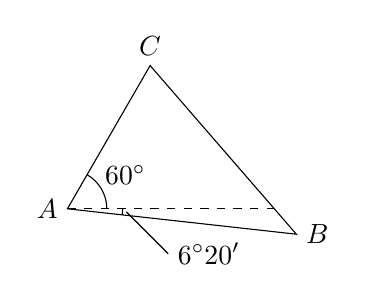
\begin{tikzpicture}[scale = 1.5]
        \draw (0,0) node [left] {$A$} coordinate (A);
        \draw (60:1.4) node [above] {$C$} coordinate (C);
        \draw ({-6-1/3}:1.95) node [right] {$B$} coordinate (B);
        \draw (A) -- (B) -- (C) -- cycle;
        \path [name path = dashedline] (A) --++ (1.9,0);
        \path [name path = BC] (B) -- (C);
        \path [name intersections = {of = dashedline and BC, by = D}];
        \draw [dashed] (A) -- (D);
        \draw (A) pic ["$60^\circ$",draw, angle eccentricity = 1.7] {angle = D--A--C};
        \draw (A) pic [draw, angle radius = 0.7cm] {angle = B--A--D};
        \draw (-3:0.5) --++ (-45:0.5) node [right] {$6^\circ 20'$};
    \end{tikzpicture}
\end{center}
\item 在$\triangle ABC$中, 若$\sqrt 3a=2b\sin A$, 求$B$.
\item 已知$\triangle ABC$的面积$S=\dfrac{b^2+c^2-a^2}4$, 求$A$.
\item 在$\triangle ABC$中, 已知$a=13$, $b=14$, $c=15$.\\
(1) 求$\cos A$;\\
(2) 求$\triangle ABC$的面积$S$.
\item 已知三角形两边之和为$8$, 其夹角为$60^\circ$. 分别求这个三角形周长的最小值和面积的最大值, 并指出面积最大时三角形的形状.
\item 求分别满足下列条件的角:\\
(1) $\sin x=\dfrac 25$, $x\in [0, \pi]$;\\
(2) $\cos x=-\dfrac 23$, $x\in [0, 2\pi ]$;\\
(3) $\tan x=-\dfrac 12$, $x\in \mathbf{R}$.
\item 在$\triangle ABC$中, $A=60^\circ$, $b=1$, 且其面积为$\sqrt 3$. 求$a$.
\item 某船在海面$A$处测得灯塔$C$在北偏东$30^\circ$方向, 与$A$相距$10\sqrt 3$海里, 且测得灯塔$B$在北偏西$75^\circ$方向, 与$A$相距$15\sqrt 6$海里. 船由$A$向正北方向航行到$D$处, 测得灯塔$B$在南偏西$60^\circ$方向. 这时灯塔$C$与$D$相距多少海里? $C$在$D$的什么方向? 
\item 如图, 为了测定对岸$A$、$B$两点之间的距离, 在河的一岸定一条基线$CD$, 测得$CD=100\text{m}$, $\angle ACD=80^\circ$, $\angle BCD=45^\circ$, $\angle BDC=70^\circ$, $\angle ADC=33^\circ$. 求$A$、$B$间的距离. (结果精确到$0.01\text{m}$)
\begin{center}
    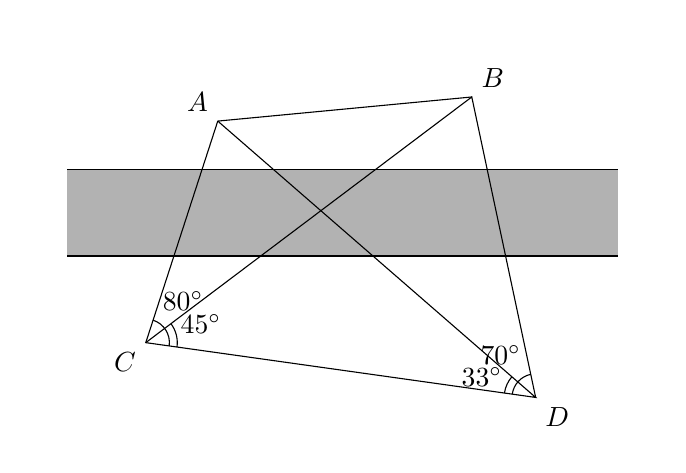
\begin{tikzpicture}
        \clip (-1.5,-1.3) rectangle (6.5,4);
        \fill [gray!60] (-1,1.1) rectangle (6,2.2);
        \draw (0,0) node [below left] {$C$} coordinate (C) ++ (-8:5) node [below right] {$D$} coordinate (D);
        \path [name path = lineBC] (C) --++ (37:10);
        \path [name path = lineBD] (D) --++(102:10);
        \path [name intersections={of = lineBC and lineBD, by=B}];
        \draw (C) -- (B) node [above right] {$B$} --(D);
        \path [name path = lineAC] (C) --++ (72:10);
        \path [name path = lineAD] (D) --++(139:10);
        \path [name intersections={of = lineAC and lineAD, by=A}];
        \draw (B) -- (A) -- (C) -- (D) -- (A) node [above left] {$A$};
        \draw (C) ++ (-8:0.3) arc (-8:72:0.3) node [above right] {$80^\circ$};
        \draw (C) ++ (-8:0.4) arc (-8:37:0.4) node [right] {$45^\circ$};
        \draw (D) ++ (172:0.4) arc (172:139:0.4) node [left] {$33^\circ$};
        \draw (D) ++ (172:0.3) arc (172:102:0.3) node [above left] {$70^\circ$};
        \draw (-1,1.1) -- (6,1.1) (-1,2.2) -- (6,2.2);
    \end{tikzpicture}
\end{center}
\item 在$\triangle ABC$中, 求证:\\
(1) $\dfrac{\cos 2A}{a^2} -\dfrac{\cos 2B}{b^2} =\dfrac1{a^2}-\dfrac 1{b^2}$;\\
(2) $(a^2-b^2-c^2)\tan A+(a^2-b^2+c^2)\tan B=0$.
\item 作出下列函数的大致图像:\\
(1) $y=1+\sin x$, $x\in [0, 2\pi ]$;\\
(2) $y=|\sin x|$, $x\in \mathbf{R}$.
\item 求下列函数的最小正周期:\\
(1) $y=1+\sin \dfrac 27x$, $x\in \mathbf{R}$;\\
(2) $y=\dfrac 13\sin (-3x+\dfrac \pi 3)$, $x\in \mathbf{R}$.
\item 已知函数$y=2\sin (2\omega x-\dfrac \pi 4)$(其中常数$\omega \ne 0$)的最小正周期为$2$, 求$\omega$的值.
\item 求下列函数的最大值和最小值, 并指出使其取得最大值和最小值时的所有$x$值的集合:\\
(1) $y=2-3\sin x$, $x\in \mathbf{R}$;\\
(2) $y=-\sin^2x+2\sin x+2$, $x\in \mathbf{R}$;\\
(3) $y=2\sin x-5$, $x\in [-\dfrac \pi 3, \dfrac{5\pi} 6]$;\\
(4) $y=\cos^2x-\sin x$, $x\in \mathbf{R}$.
\item 判断下列函数的奇偶性, 并说明理由:\\
(1) $y=-2\sin x$;\\
(2) $y=\dfrac{\sin x}x$;\\
(3) $y= \dfrac x{1+\sin x}$.
\item 利用函数的单调性, 比较下列各组数的大小:\\
(1) $\sin \dfrac{3\pi} 11$与$\sin \dfrac{5\pi} 12$;\\
(2) $\sin (-\dfrac{76\pi}{11})$与$\sin \dfrac{85\pi}{12}$.
\item  求下列函数的单调区间:\\
(1) $y=2-\sin x$;\\
(2) $y=3\sin (\dfrac x3+\dfrac \pi 4)$.
\item 求下列函数的值域:\\
(1) $y=3\sin x+\sqrt 3\cos x$;\\
(2) $y=\sin^2x+4\sin x$.
\item 求函数$y=2\sin x-1$的零点.
\item 可以利用正弦函数$y=\sin x$和$y=\dfrac 12$的图像, 并结合正弦函数的周期性来求解不等式$\sin x\ge\dfrac 12$. 请根据上述方法求函数$y=\sqrt{2\sin x-1}$的定义域.
\item 求函数$y=\sin \dfrac x2+\cos \dfrac x2$的单调减区间.
\item 已知函数$y=\dfrac{\sqrt 3}2\sin 2kx+\cos^2kx$(其中常数$k>0$)的最小正周期为$\pi$, 求$k$的值.
\item 求函数$y=\sin (x+\dfrac \pi 6)$, $x\in [-\dfrac\pi 3, \dfrac \pi 2]$的值域.
\item 求函数$y=\sin^4x+\cos^4x$的最小正周期与最值.
\item 设半圆$O$的直径为$2$, 而$A$为直径延长线上的一点, 且$OA=2$. 对半圆上任意给定的一点$B$, 以$AB$为一边作等边三角形$ABC$, 使$\triangle ABC$和$\triangle ABO$在$AB$的两侧(如图所示). 求四边形$OACB$面积的最大值, 并求使四边形$OACB$面积取得最大值时的$\angle AOB$的大小.
\begin{center}
    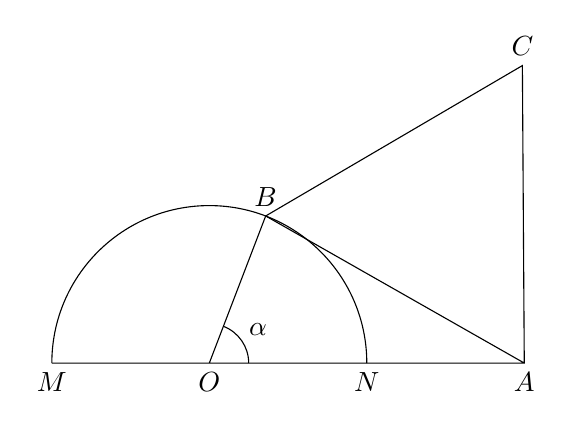
\begin{tikzpicture}[scale = 2]
        \draw (-1,0) node [below] {$M$} coordinate (M);
        \draw (1,0) node [below] {$N$} coordinate (N);
        \draw (0,0) node [below] {$O$} coordinate (O);
        \draw (2,0) node [below] {$A$} coordinate (A);
        \draw (0.358,0.934) node [above] {$B$} coordinate (B);
        \draw (1.988,1.889) node [above] {$C$} coordinate (C);
        \draw (M) -- (A) -- (C) -- (B) -- (O) (B) -- (A);
        \draw (N) arc (0:180:1);
        \draw (O) pic ["$\alpha$",draw,angle eccentricity = 1.5] {angle = A--O--B};
    \end{tikzpicture}
\end{center}
\item 如图, 函数$y=f(x)$($x\in\mathbf{R}$)的图像由折线段组成, 且当$x$取偶数时, 对应的$y$的值为$0$; 而当$x$取奇数时, 对应的$y$的值为$2$.
\begin{center}
    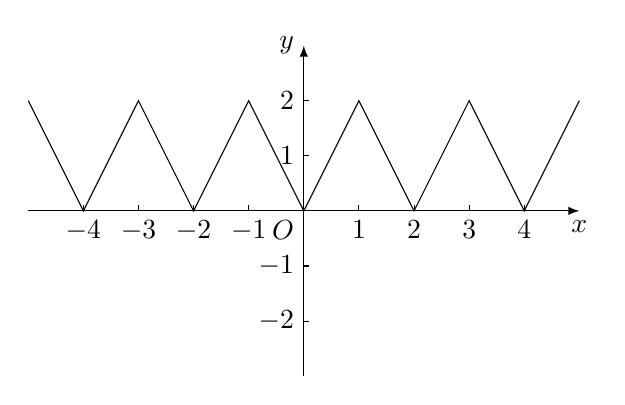
\begin{tikzpicture}[>=latex,scale = 0.7]
        \draw [->] (-5,0) -- (5,0) node [below] {$x$};
        \draw [->] (0,-3) -- (0,3) node [left] {$y$};
        \draw (0,0) node [below left] {$O$};
        \foreach \i in {-4,-3,-2,-1,1,2,3,4}
        {\draw (\i,0.1) -- (\i,0) node [below] {$\i$};};
        \foreach \i in {-2,-1,1,2}
        {\draw (0.1,\i) -- (0,\i) node [left] {$\i$};};
        \draw (-5,2) -- (-4,0) -- (-3,2) -- (-2,0) -- (-1,2) -- (0,0) -- (1,2) -- (2,0) -- (3,2) -- (4,0) -- (5,2);
    \end{tikzpicture}
\end{center}
(1) 写出函数$y=f(x)$的最小正周期;\\
(2) 作出函数$y=f(x-1)$的图像.
\item 作出下列函数的大致图像:\\
(1) $y=2\cos x-1$, $x\in [0, 2\pi ]$;\\
(2) $y=|\cos x|$, $x\in \mathbf{R}$.
\item 求下列函数的最小正周期:\\
(1) $y=\cos \dfrac x3$;\\
(2) $y=2\cos (-2x+\dfrac \pi 6)$.
\item 求下列函数的最大值和最小值, 并指出使其取得最大值和最小值时$x$的集合:\\
(1) $y=3^{\cos 2x}$, $x\in \mathbf{R}$;\\
(2) $y=\cos x-\sin^2x$, $x\in \mathbf{R}$.
\item 判断下列函数的奇偶性, 并说明理由:\\
(1) $y=\sin^2x+\cos x$;\\
(2) $y=2\sin x+\cos 2x$;\\
(3) $y=\dfrac x{1+\cos x}$.
\item 求函数$y=\cos 2x$, $x\in [-\dfrac \pi 6, \dfrac{2\pi} 3]$的单调区间和值域.
\item 函数$y=1-2\sin^2(x-\dfrac \pi 4)$是\bracket{20}.
\twoch{最小正周期为$\pi$的奇函数}{最小正周期为$\pi$的偶函数}{最小正周期为$\dfrac \pi 2$的奇函数}{最小正周期为$\dfrac \pi 2$的偶函数}
\item 设函数$y=\sin (\dfrac x2+\varphi)$(其中常数$\varphi \in [0, \pi ]$)是$\mathbf{R}$上的偶函数, 求$\varphi$的值.
\item 已知$y=\sin x$和$y=\cos x$的图像的连续三个交点$A$、$B$、$C$构成$\triangle ABC$, 求$\triangle ABC$的面积.
\item 当函数$y=A\sin (\omega x+\varphi)$($A>0$, $\omega >0$)中的常数$A$、$\omega$、$\varphi$分别取下列各组值时, 在同一平面直角坐标系中分别作出它们的图像:\\
(1) $A=\dfrac 12$, $\omega =1$, $\varphi =0$;\\
(2) $A=1$, $\omega =\dfrac 12$, $\varphi =0$;\\
(3) $A=1$, $\omega =1$, $\varphi =-\dfrac \pi 2$.
\item 求函数$y=\sqrt 2\sin (30\pi x-\dfrac\pi{12})$的振幅、频率和初始相位.
\item 已知某交流电流$I$($\text{A}$)随时间$t$($\text{s}$)的变化规律可以用函数$I=8\sin (100\pi t-\dfrac \pi 2)$, $t\in [0, +\infty)$表示. 求这种交流电流在$0.5\text{s}$内往复运行的次数.
\item 作出函数$y=2\sin (\dfrac 12x+\dfrac \pi 6)$的大致图像.
\item 如图, 弹簧挂着的小球上下振动. 设小球相对于平衡位置(即静止时的位置)的距离$h$($\text{cm}$)与时间$t$($\text{s}$)之间的函数表达式是$h=2\sin (\pi t+\dfrac\pi 4)$, $t\ge 0$, 作出这个函数的大致图像, 并回答下列问题:
\begin{center}
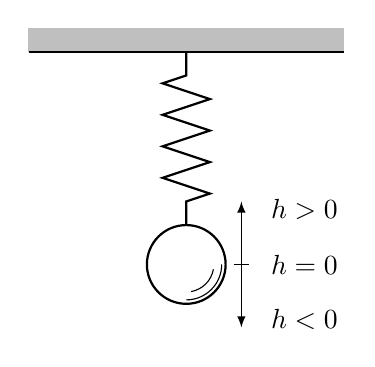
\begin{tikzpicture}[>=latex]
\draw [thick] (0,0) circle (0.5);
\draw (0.45,0) arc (0:-90:0.45);
\draw (-10:0.35) arc (-10:-80:0.35);
\draw [thick] (0,0.5) -- (0,0.8) -- (0.3,0.9) -- (-0.3,1.1) -- (0.3,1.3) -- (-0.3,1.5) -- (0.3,1.7) -- (-0.3,1.9) -- (0.3,2.1) -- (-0.3,2.3) -- (0,2.4) -- (0,2.7);
\filldraw [gray!50] (-2,2.7) rectangle (2,3);
\draw [thick] (-2,2.7) -- (2,2.7);
\draw (0.6,0) -- (0.8,0);
\draw [->] (0.7,0) -- (0.7,0.8);
\draw [->] (0.7,0) -- (0.7,-0.8);
\draw (1.5,0) node {$h=0$};
\draw (1.5,0.7) node {$h>0$};
\draw (1.5,-0.7) node {$h<0$};
\end{tikzpicture}
\end{center}
(1) 小球开始振动(即$t=0$)时的位置在哪里?\\
(2) 小球最高点和最低点与平衡位置的距离分别是多少?\\
(3) 经过多少时间小球往复振动一次?\\
(4) 每秒钟小球往复振动多少次?
\item 作出函数$y=\sin x+\sqrt 3\cos x$的大致图像.
\item 如图, 已知函数$y=A\cos (\omega x+\varphi)$($A>0$, $\omega >0$, $0<\varphi <2\pi$)的图像与$y$轴的交点为$(0, 1)$, 并已知其在$y$轴右侧的第一个最高点和第一个最低点的坐标分别为$(x_0, 2)$和$(x_0+2\pi , -2)$. 求此函数的表达式.
\begin{center}
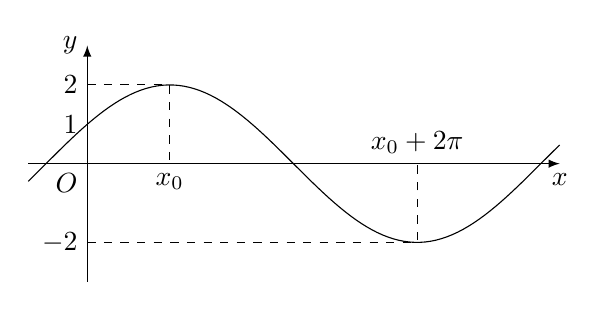
\begin{tikzpicture}[>=latex,scale = 0.5]
\draw [->] (-1.5,0) -- (12,0) node [below] {$x$};
\draw [->] (0,-3) -- (0,3) node [left] {$y$};
\draw (0,0) node [below left] {$O$};
\draw [domain = -1.5:12, samples = 100] plot (\x,{2*sin(\x/2/pi*180+30)});
\foreach \i in {-2,1,2} {\draw (0,\i) node [left] {$\i$};};
\draw [dashed] (0,2) -- ({2*pi/3},2) -- ({2*pi/3},0) node [below] {$x_0$};
\draw [dashed] (0,-2) -- ({2*pi/3+2*pi},-2) -- ({2*pi/3+2*pi},0) node [above] {$x_0+2\pi$};
\end{tikzpicture}
\end{center}
\item 三相交流电的插座上有四个插孔, 其电压分别为$U_0=0$, $U_1=A\sin \omega t$, $U_2=A\sin (\omega t+\dfrac{2\pi} 3)$, $U_3=A\sin (\omega t+\dfrac{4\pi} 3)$, 其中$\omega =100\pi\text{rad}/\text{s}$, $A=220\sqrt 2\text{V}$. 记$U_2-U_1$, $U_3-U_2$, $U_1-U_3$的最大值分别为$Y_1$、$Y_2$、$Y_3$, 试计算三相交流电的线电压的有效值$\dfrac{Y_1}{\sqrt 2}$、$\dfrac{Y_2}{\sqrt 2}$及$\dfrac{Y_3}{\sqrt 2}$.
\item 求下列函数的最小正周期:\\
(1) $y=\tan (-\dfrac 12x)$;\\
(2) $y=\tan (3x+\dfrac \pi 3)$.
\item 求函数$y=\tan (ax+b)$($a$、$b$为常数, 且$a\ne 0$)的最小正周期.
\item 求函数$y=\tan x$, $x\in  [-\dfrac \pi 3, \dfrac \pi 4]$的最大值和最小值, 并指出使其取得最大值和最小值时所有$x$的值.
\item 判断下列函数的奇偶性, 并说明理由:\\
(1) $y=\tan 2x$;\\
(2) $y=|\tan x|$;\\
(3) $y= \dfrac 1{\tan x}$;\\
(4) $y=\dfrac{\tan x}x$.
\item 求函数$y=2\tan (3x-\dfrac \pi 6)$的定义域和单调区间.
\item 求正切函数$y=\tan x$的零点.
\item 对于函数$y=f(x)$, 其中$f(x)=a\sin 2x+b\tan x+3$, 已知$f(-2)=1$. 求$f(\pi +2)$的值.
\item 求函数$y=\tan^2 x-\tan x$, $x\in  [-\dfrac \pi 4, \dfrac \pi 4]$的最大值与最小值.
\item 如果把平面上所有的单位向量的起点都平移到同一点, 那么它们的终点构成的图形是什么?
\item 在平面直角坐标系中, 作出表示下列向量的有向线段:\\
(1) 向量$\overrightarrow a$的起点在坐标原点, 与$x$轴正方向的夹角为$120^\circ$且$|\overrightarrow a|=3$;\\
(2) 向量$\overrightarrow b$的模为$4$, 方向与$y$轴的正方向反向;\\
(3) 向量$\overrightarrow c$的方向与$y$轴的正方向同向, 模为$2$.
\item 判断下列命题的真假, 并说明理由:\\
(1) 长度相等的向量均为相等向量;\\
(2) 给定向量$\overrightarrow a$、$\overrightarrow b$、$\overrightarrow c$, 若$\overrightarrow a=\overrightarrow b$, $\overrightarrow b=\overrightarrow c$, 则$\overrightarrow a=\overrightarrow c$;\\
(3) 若$ABCD$为平行四边形, 则必有$\overrightarrow{AB}=\overrightarrow{CD}$;\\
(4) 若平面上四点$A$、$B$、$C$、$D$使$\overrightarrow{AB}=\overrightarrow{CD}$, 则$AB\parallel CD$.
\item 如图, 在$\triangle ABC$中, 点$D$、$E$、$F$分别是$AB$、$BC$、$CA$的中点, 根据下列条件, 写出相应的向量:
\begin{center}
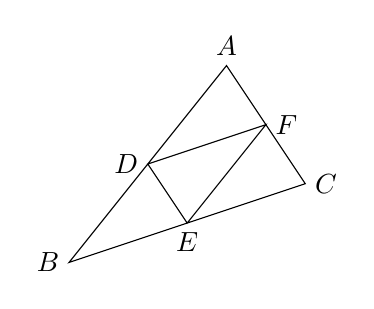
\begin{tikzpicture}[>=latex]
\draw (0,0) node [left] {$B$} coordinate (B);
\draw (3,1) node [right] {$C$} coordinate (C);
\draw (2,2.5) node [above] {$A$} coordinate (A);
\draw ($(A)!0.5!(B)$) node [left] {$D$} coordinate (D);
\draw ($(B)!0.5!(C)$) node [below] {$E$} coordinate (E);
\draw ($(A)!0.5!(C)$) node [right] {$F$} coordinate (F);
\draw (A) -- (B) -- (C) -- cycle (D) -- (E) -- (F) -- cycle;
\end{tikzpicture}
\end{center}
(1) 与向量$\overrightarrow{AD}$相等的向量;\\
(2) 向量$\overrightarrow{DE}$的负向量;\\
(3) 与向量$\overrightarrow{EF}$平行的向量.
\item 如图, 已知向量$\overrightarrow a$、$\overrightarrow b$、$\overrightarrow c$, 作出下列向量:\\
\begin{center}
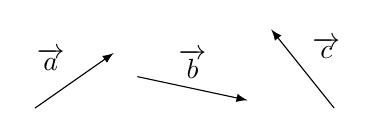
\begin{tikzpicture}[>=latex]
\draw [->] (0,0) -- (1,0.7);
\draw (0.5,0.35) node [above left] {$\overrightarrow a$};
\draw [->] (1.3,0.4) -- (2.7,0.1);
\draw (2,0.25) node [above] {$\overrightarrow b$};
\draw [->] (3.8,0) -- (3,1);
\draw (3.4,0.5) node [above right] {$\overrightarrow c$};
\end{tikzpicture}
\end{center}
(1) $\overrightarrow a+\overrightarrow b$, $\overrightarrow b+\overrightarrow c$, $\overrightarrow a+\overrightarrow c$;\\
(2) $(\overrightarrow a+\overrightarrow b)+\overrightarrow c$和$\overrightarrow a+(\overrightarrow b+\overrightarrow c)$.
\item 化简下列向量运算:\\
(1) $\overrightarrow{AB}+\overrightarrow{BC}+\overrightarrow{CD}+\overrightarrow{DA}$;\\
(2) $(\overrightarrow{AB}-\overrightarrow{AC})+(\overrightarrow{BD}-\overrightarrow{CD})$;\\
(3) $(\overrightarrow{AB}+\overrightarrow{MB})+(\overrightarrow{BD}+\overrightarrow{DM})$.
\item 设向量$\overrightarrow a$表示``向东走$2\text{km}$''; 向量$\overrightarrow b$表示``向西走$1\text{km}$''; 向量$\overrightarrow c$表示``向南走$2\text{km}$''; 向量$\overrightarrow d$表示``向北走$1\text{km}$''. 试说明下列向量所表示的意义:\\
(1) $\overrightarrow a+\overrightarrow a$;\\
(2) $\overrightarrow a+\overrightarrow c$;\\
(3) $\overrightarrow a+\overrightarrow b+\overrightarrow d$;\\
(4) $\overrightarrow c+\overrightarrow d+\overrightarrow c$.
\item 设向量$\overrightarrow{OA}=\overrightarrow a$, $\overrightarrow{OB}=\overrightarrow b$, 且$|\overrightarrow{OA}|=12$,$|\overrightarrow{OB}|=4$, $\angle AOB=\dfrac \pi 3$. 求$|\overrightarrow a+\overrightarrow b|$.
\item 运用作图的方法, 验证下列等式:\\
(1) $\dfrac 12(\overrightarrow a+\overrightarrow b)+\dfrac 12(\overrightarrow a-\overrightarrow b)=\overrightarrow a$;\\
(2) $\dfrac 12(\overrightarrow a+\overrightarrow b)-\dfrac 12(\overrightarrow a-\overrightarrow b)=\overrightarrow b$.
\item 化简下列向量运算:\\
(1) $4(\overrightarrow a+\overrightarrow b)-3(\overrightarrow a-\overrightarrow b)-8\overrightarrow b$;\\
(2) $3(\overrightarrow a-2\overrightarrow b+\overrightarrow c)+4(\overrightarrow c-\overrightarrow a-\overrightarrow b)$;\\
(3) $\dfrac 13[\dfrac 12(2\overrightarrow a+8\overrightarrow b)-(4\overrightarrow a-2\overrightarrow b)]$.
\item 已知四边形$ABCD$和点$O$在同一平面上, 设向量$\overrightarrow{OA}=\overrightarrow a$, $\overrightarrow{OB}=\overrightarrow b$, $\overrightarrow{OC}=\overrightarrow c$, $\overrightarrow{OD}=\overrightarrow d$, 且$\overrightarrow a+\overrightarrow c=\overrightarrow b+\overrightarrow d$. 求证: $ABCD$是平行四边形.
\item 已知平行四边形$ABCD$, 设向量$\overrightarrow{AC}=\overrightarrow a$, $\overrightarrow{BD}=\overrightarrow b$. 试用$\overrightarrow a$、$\overrightarrow b$表示下列向量:\\
(1) $\overrightarrow{AB}$;\\
(2) $\overrightarrow{BC}$.
\item 如图是由边长为$1$的小正方形组成的网格. 按要求, 分别以$A$、$B$、$C$为向量的起点, 在图中画出下列向量:
\begin{center}
\begin{tikzpicture}[>=latex,scale = 0.5]
\foreach \i in {0,1,...,9} {\draw [dashed] (\i,0) -- (\i,8);};
\foreach \i in {0,1,...,8} {\draw [dashed] (0,\i) -- (9,\i);};
\draw [->] (10,5) -- (10,8) node [right] {北};
\filldraw (1,2) circle (0.1) node [below left] {$A$};
\filldraw (7,3) circle (0.1) node [below left] {$B$};
\filldraw (3,5) circle (0.1) node [above left] {$C$};
\end{tikzpicture}
\end{center}
(1) 正北方向且模为$2$的向量$\overrightarrow{AE}$;\\
(2) 模为$2\sqrt 2$、方向为北偏西$45^\circ$的向量$\overrightarrow{BF}$;\\
(3) (2)中向量$BF$的负向量.
\item 已知正方形$ABCD$的边长为$1$, 求:\\
(1) $|\overrightarrow{AB}+\overrightarrow{BC}|$;\\
(2) $|\overrightarrow{AB}+\overrightarrow{BD}-\overrightarrow{AC}|$;\\
(3) $|\overrightarrow{AB}-\overrightarrow{BC}+\overrightarrow{AC}|$.
\item 如图, 已知向量$\overrightarrow a$、$\overrightarrow b$、$\overrightarrow c$, 作出下列向量:
\begin{center}
\begin{tikzpicture}[>=latex]
\draw [->] (0,0) -- (1,0.7);
\draw (0.5,0.35) node [above left] {$\overrightarrow a$};
\draw [->] (1.3,-0.7) -- (2.5,-0.7);
\draw (1.9,-0.7) node [above] {$\overrightarrow b$};
\draw [->] (2.9,0.3) -- (3.9,-0.4);
\draw (3.4,-0.05) node [above right] {$\overrightarrow c$};
\end{tikzpicture}
\end{center}
(1) $\overrightarrow a+\overrightarrow c-\overrightarrow b$和$\overrightarrow a+(\overrightarrow c-\overrightarrow b)$;\\
(2) $\overrightarrow a-(\overrightarrow b+\overrightarrow c)$和$\overrightarrow a-\overrightarrow c-\overrightarrow b$.
\item 试用作图法验证下列不等式:\\
(1) $|\overrightarrow a|-|\overrightarrow b|\le|\overrightarrow a+\overrightarrow b|\le|\overrightarrow a|+|\overrightarrow b|$;\\
(2) $|\overrightarrow a|-|\overrightarrow b|\le|\overrightarrow a-\overrightarrow b|\le|\overrightarrow a|+|\overrightarrow b|$.
\item 判断下列命题的真假, 并说明理由:\\
(1) 若存在一个$\lambda \in \mathbf{R}$使$\lambda \overrightarrow a=\lambda \overrightarrow b$, 则$\overrightarrow a=\overrightarrow b$;\\
(2) 对于任意给定的实数$\lambda$和向量$\overrightarrow a$、$\overrightarrow b$, 均有$\lambda (\overrightarrow a-\overrightarrow b)=\lambda \overrightarrow a-\lambda \overrightarrow b$;\\
(3) 对于任意给定的实数$\lambda$、$\mu$和向量$\overrightarrow a$, 均有$(\lambda -\mu)\overrightarrow a=\lambda \overrightarrow a-\mu\overrightarrow a$.
\item 设$\overrightarrow a$、$\overrightarrow b$是两个不平行的向量, 求证: 若实数$\lambda$、$\mu$使得$\lambda \overrightarrow a+\mu\overrightarrow b=0$, 则$\lambda =\mu=0$.
\item 已知$\overrightarrow {e_1}$、$\overrightarrow {e_2}$是两个不平行的向量, 而向量$\overrightarrow{AB}=3\overrightarrow {e_1}-2\overrightarrow {e_2}$, $\overrightarrow{BC}=-2\overrightarrow {e_1}+4\overrightarrow {e_2}$, $\overrightarrow{CD}=-2\overrightarrow {e_1}-4\overrightarrow {e_2}$. 求证: $A$、$C$、$D$三点共线.
\item 已知$G$是$\triangle ABC$的重心, $D$、$E$、$F$分别为$AB$、$AC$、$BC$中点. 求证: $\overrightarrow{GD}+\overrightarrow{GE}+\overrightarrow{GF}=\overrightarrow 0$.
\item 设向量$\overrightarrow a$、$\overrightarrow b$满足$|\overrightarrow a|=6$, $|\overrightarrow b|=3$, 且$\overrightarrow a\cdot \overrightarrow b=-12$, 则向量$\overrightarrow a$在向量$\overrightarrow b$方向上的投影是\blank{50}.
\item 在$\triangle ABC$中, 若$|ABC|=3$, $|AC|=2$, $|BC|=\sqrt {10}$, 则$\overrightarrow{AB}\cdot \overrightarrow{AC}=$\blank{50}.
\item 已知向量$\overrightarrow a$与$\overrightarrow b$的夹角为$45^\circ$, 且$|\overrightarrow a|=1,|2\overrightarrow a-\overrightarrow b|=\sqrt {10}$, 则$|\overrightarrow b|=$\blank{50}.
\item 在菱形$ABCD$中, $(\overrightarrow{AB}+\overrightarrow{AD})\cdot (\overrightarrow{AB}-\overrightarrow{AD})=$\blank{50}.
\item 设向量$\overrightarrow a$、$\overrightarrow b$满足$|\overrightarrow a|=1$, $|\overrightarrow b|=\sqrt 2$, 向量$\overrightarrow a-\overrightarrow b$与$\overrightarrow a$垂直. 求$\langle \overrightarrow a, \overrightarrow b\rangle$.
\item 设向量$\overrightarrow a$、$\overrightarrow b$满足$\langle \overrightarrow a, \overrightarrow b\rangle =60^\circ$, $|\overrightarrow a|=3$, $|\overrightarrow b|=3$. 求$(\overrightarrow a+\overrightarrow b)^2$.
\item 在$\triangle ABC$中, $|AB|=|AC|=4$, $\overrightarrow{AB}\cdot \overrightarrow{AC}=8$. 判断$\triangle ABC$的形状, 并说明理由.
\item 设向量$\overrightarrow a$、$\overrightarrow b$满足$|\overrightarrow a|=4$, $|\overrightarrow b|=5$, $|\overrightarrow a+\overrightarrow b|=\sqrt{21}$. 分别求下列各式的值:\\
(1) $\overrightarrow a\cdot \overrightarrow b$;\\
(2) $(2\overrightarrow a-\overrightarrow b)\cdot (\overrightarrow a+3\overrightarrow b)$.
\item 设$\overrightarrow{e_1}$、$\overrightarrow{e_2}$是互相垂直的单位向量, 向量$\overrightarrow a=2\overrightarrow{e_1}-\overrightarrow{e_2}$, $\overrightarrow b=-3\overrightarrow{e_1}+2\overrightarrow {e_2}$. 求$(\overrightarrow a-2\overrightarrow b)\cdot (\overrightarrow a+\overrightarrow b)$.
\item 设向量$\overrightarrow a$、$\overrightarrow b$满足$|\overrightarrow a|=1$, $(\overrightarrow a+\overrightarrow b)\cdot 
(\overrightarrow a-\overrightarrow b)=\dfrac 12$.\\
(1) 求$|\overrightarrow b|$;\\
(2) 设$\overrightarrow a\cdot \overrightarrow b=\dfrac 12$, 求$\langle \overrightarrow a, \overrightarrow b\rangle$.
\item 设向量$\overrightarrow a$、$\overrightarrow b$、$\overrightarrow c$满足$\overrightarrow a+\overrightarrow b+\overrightarrow c=\overrightarrow 0$, 且$|\overrightarrow a|=4$, $|\overrightarrow b|=3$, $|\overrightarrow c|=5$. 求下列各式的值:\\
(1) $\overrightarrow a\cdot \overrightarrow c$;\\
(2) $\overrightarrow a\cdot \overrightarrow b+\overrightarrow b\cdot \overrightarrow c+\overrightarrow c\cdot \overrightarrow a$.
\item 在$\triangle ABC$中, $C=\dfrac \pi 2$,  $|AC|=1$. 求$\overrightarrow{AB}\cdot \overrightarrow{CA}$.
\item 在$\triangle$ $ABC$中, 若$|AB|=2$, $|AC|=3$, $\overrightarrow{AB}\cdot \overrightarrow{BC}=1$, 则$|BC|=$\blank{50}.
\item 设向量$\overrightarrow a$、$\overrightarrow b$满足$|\overrightarrow a|=2$, $|\overrightarrow b|=1$, $\langle \overrightarrow a, \overrightarrow b\rangle =\dfrac{2\pi} 3$. 求$|\overrightarrow a-\overrightarrow b|$.
\item 在$\triangle ABC$中, $|BC|=3$, $|AC|=1$, $\angle BCA=30^\circ$. 求$\overrightarrow{BC}\cdot \overrightarrow{CA}$.
\item 在直角三角形$ABC$中, 若$D$是斜边$AB$的中点, $P$为线段$CD$的中点, 则$\dfrac{|\overrightarrow{PA}|^2+|\overrightarrow{PB}|^2}{|\overrightarrow{PC}|^2}=$\blank{50}.
\item 在$\triangle ABC$中, 设$M$是$BC$的中点, 且$|AM|=3$, $|BC|=10$, 则$\overrightarrow{AB}\cdot \overrightarrow{AC}=$\blank{50}.
\item 已知$\overrightarrow a$、$\overrightarrow b$都是非零向量, 且$\overrightarrow a+3\overrightarrow b$与$7\overrightarrow a-5\overrightarrow b$垂直, $\overrightarrow a-4\overrightarrow b$与$7\overrightarrow a-2\overrightarrow b$垂直. 求$\overrightarrow a$、$
\overrightarrow b$的夹角.
\item 在$\triangle ABC$中, 内角$A$、$B$、$C$的对边依次为$a$、$b$、$c$. 求证: $\overrightarrow{AB}\cdot \overrightarrow{AC}=\dfrac 12(b^2+c^2-a^2)$.
\item 在四边形$ABCD$中, 设向量$\overrightarrow{AB}=\overrightarrow a$, $\overrightarrow{BC}=\overrightarrow b$, $\overrightarrow{CD}=\overrightarrow c$, $\overrightarrow{DA}=\overrightarrow d$, 且$\overrightarrow a\cdot \overrightarrow b=\overrightarrow b\cdot
\overrightarrow c=\overrightarrow c\cdot \overrightarrow d=\overrightarrow d\cdot \overrightarrow a$. 求证: 四边形$ABCD$是矩形.



\iffalse

\item 如图, $OADB$是以向量$OA=\overrightarrow a, OB=\overrightarrow b$为邻边的平行四边形, $C$是对角线的交点, 且$BM=13BC, CN=13CD$. 试用$\overrightarrow a$、$\overrightarrow$ $b$表示$OM$、$ON$、$MN$.
\item 已知向量$\overrightarrow a=(-1, 2), \overrightarrow b=(2, 1)$. 求$2\overrightarrow a+3\overrightarrow b, \overrightarrow a-2\overrightarrow b, 12\overrightarrow a-13\overrightarrow b$.
\item 已知点$A(3, 2)$、$B(7, 5)$、$C(-1, 8)$, 求$AB-12AC$.
\item 已知向量$\overrightarrow a=(-5, 12)$, 求$|\overrightarrow a|$以及向量$\overrightarrow a$的单位向量珬$a0$.
\item 已知点$A(1, 2)$、$B(-3, 1)$, 且$AC=12AB, AD=3AB, AE=-13A}{$求点$C$、$D$、$E$的坐标.
\item 已知向量$\overrightarrow a=(5, 3), \overrightarrow b=(x, 1)$, 且$\overrightarrow a\parallel \overrightarrow b$. 求实数$x$的值.
\item 已知点$A(3, 0)$、$B(-1, -6)$, 点$P$是直线$AB$上一点, 且$|AP|=13|AB|$. 求点$P$的坐标.
\item 已知向量$\overrightarrow a=(3, -1), \overrightarrow b=(1, -2)$. 求$\overrightarrow a\cdot \overrightarrow b$与$\langle$ $\overrightarrow a, \overrightarrow b\rangle$.
\item 已知向量$\overrightarrow a=(3-m, 3m), \overrightarrow b=(m+2, -2)$, 且$\overrightarrow a\perp \overrightarrow b$. 求实数$m$的值.
\item 已知向量$\overrightarrow a=(2, 4)$, 求与$\overrightarrow a$垂直的单位向量的坐标.B组$
\item$已知$O$为坐标原点, 在$\triangle ABC$中, 向量$OA=(2, 3), OB=(1, 4)$, 且$OC=3OA, OD=3OB, OE=2OA+OB$. 求$C$、D、$E$三点的坐标, 并判断$C$、D、$E$三点是否共线. $2$. 已知向量$\overrightarrow a=(1, 2), \overrightarrow b=(m, 1)$, 且$\overrightarrow a+2\overrightarrow b$与$2\overrightarrow$ $a-\overrightarrow b$平行. 求实数$m$的值.
\item 经过点$M(-2, 3)$的直线分别与$x$轴、$y$轴交于$A$、B两点, 且$|AB|=3|AM|$.求点$A$、B的坐标.
\item 已知向量$\overrightarrow a=(1, -1), \overrightarrow b=(2, -3)$, 且$k\overrightarrow a-2\overrightarrow b$与$\overrightarrow a$垂直. 求实数$k$的值.

\item$已知平面上$A$、B两点的坐标分别是$(3, 5)$、$(0, 1), P$为直线$AB$上一点, 且$AP=15PB$. 求点$P$的坐标.
\item 已知$\triangle ABC$的三个顶点$A$、B、$C$的坐标分别是$(1, 2)$、$(2, 3)$、$(3, 7)$, 求此三角形的面积.
\item 用向量方法证明三角形的余弦定理.
(第$5$题$)$
\item 菱形是四条边都相等的四边形. 用向量方法证明菱形的对角线互相垂直.
\item 如图, 已知$M$、$N$是平行四边形$ABCD$的对角线$AC$上的两点, 且$AM=CN$. 求证$: BMDN$是平行四边形.8平面向量$126B$组$
\item$证明:三角形的三条中线相交于一点.
\item 已知平面上不共线的三点$A(x1, y1)$、$B(x2, y2)$与$C(x3, y3)$, 求证$: \triangle ABC$的面积$S=12|x1(y2-y3)$+x2(y3-y1)+x3$(y1-y2)|$.
\item 已知$a$、b均为正数, 且$a+b=1$. 求证$: (a+2)$2+(b+3)2\ge$18$.
\item 已知$ABCD$是正方形, $M$是$AB$边的中点, 点$E$在对角线$AC$上, 且$AE: EC=3: 1$. 求证$: \angle MED=\pi 2$.
\item 用向量方法证明:把一个平行四边形的一个顶点和两条不过此顶点的边的中点分别连线, 则这两条连线三等分此平行四边形的一条对角线.

\item$已知复数$(12x+y)+(5x+23y-16)\mathrm{\mathrm{i}}=-4$, 其中$x$、$y\\mathrm{i}n R$. 求$x$、y的值.
\item 已知$(x+y)-xy\mathrm{i}=-5+24\mathrm{i}$, 其中$x$、$y\in \mathbf{R}$. 求$x$、y的值.
\item 计算:(1)$(14-135\mathrm{i})+(23+52\mathrm{i})$;
(2)$-(3-4\mathrm{i})$+(2+\mathrm{i})-$(1-5\mathrm{i})$;
(3)[(a+b)+(a-b)\mathrm{i}]-[(a-b)-(a+b)\mathrm{i}](a、$b\in \mathbf{R})$;
(4)$(4-3\mathrm{i})(3+4\mathrm{i})$;
(5)$(-2+3\mathrm{i})(5-4\mathrm{i})$;
(6)$(\sqrt 22-\sqrt 22\mathrm{i})2$;
(7)$7+9\mathrm{i}1+2\mathrm{i}$;
(8)$6-5\mathrm{i}2+3\mathrm{i}$;
(9)$\sqrt 5+\sqrt 3\mathrm{i}
\sqrt 5-\sqrt 3\mathrm{i}-\sqrt 3+\sqrt 5\mathrm{i}
\sqrt 3-\sqrt 5\mathrm{i}$.
\item 用复数乘法公式验证:若$c+d\mathrm{\mathrm{i}}\ne 0$, 则$(c+d\mathrm{\mathrm{i}})(ac+bdc2+d2+bc-adc2+d2\mathrm{i})=a+b\mathrm{i}$.
\item 已知复数$z1=(a2+2)+(-2a-1)\mathrm{\mathrm{i}}, z2=(a-6)+(a2+a)\mathrm{\mathrm{i}}$, 其中$a\\mathrm{i}n R$. 若$z1+z2=2+\mathrm{i}$, 求$a$的值.
\item 设实数$x$、y使得$(x+y\mathrm{i})$\mathrm{i}-2+4\mathrm{i}=(x-y\mathrm{i})$(1+\mathrm{i})$, 求$x$、y的值.
\item 已知实数$x$、y使得$x1-\mathrm{i}+ y1-2\mathrm{i}= 51-3\mathrm{i}$, 求$x$、y的值.
\item 求复数$-3+2\mathrm{\mathrm{i}}$与复数$2+3\mathrm{\mathrm{i}}$的乘积的共轭复数.
\item 若复数$z1=a+2\mathrm{i}(a\in \mathbf{R}), z2=3+4\mathrm{i}$, 且$z1z2$为纯虚数, 求$a$的值.
\item 已知复数$z=1+\mathrm{\mathrm{i}}$, 求$z2-z+1z2+z+1$的值.
\item 求实数$m$的值, 使得复数$(m2-3m-4)+(m2-5m-6)\mathrm{\mathrm{i}}$分别是:(1)实数;
(2)纯虚数;
(3)零.
\item 已知$(2x2-5x+2)+(y2+y-2)\mathrm{i}=0$, 其中$x$、$y\in \mathbf{R}$. 求$x$、y的值.B组$
\item$计算:(1)$(1-\mathrm{i}1+\mathrm{i})3$;
(2)$-2+2\sqrt 3\mathrm{i}
(\sqrt 3+\mathrm{i})$2 ;
(3)$(1+\mathrm{i})$10-$(1-\mathrm{i})10$.9复数$142
\item$已知复数$z1=5+10\mathrm{\mathrm{i}}$及$z2=3-4\mathrm{\mathrm{i}}$, 且复数$z$满足$1z=1z1+1z2$. 求$z$.
\item 已知复数$(x2-y2-7)+(x-y-3)\mathrm{i}$等于$-2\mathrm{i}$, 其中$x$、$y\in \mathbf{R}$. 求$x$、y的值.
\item 已知$(2x+3y)+(x2-y2)\mathrm{i}=y+2+4\mathrm{i}$, 其中$x$、$y\in \mathbf{R}$. 求$x$、y的值.
\item 是否存在实数$m$, 使得复数$z=m2+2m-15+m2-5m+6m2-25 \mathrm{i}$分别满足下列条件? 若存在, 求出$m$的值或取值范围; 若不存在, 请说明理由.
(1)$z$是实数;
(2)$z$是虚数;
(3)$z$是纯虚数;
(4)$z$是零.
\item 选择题:(1)设$z1$、$z2\in \mathbf{C}$, 则``z1、$z2$中至少有一个虚数$''$是``z1-z2为虚数$''$的$
($ $)$
\fourch{ 充分非必要条件; $}{$必要非充分条件; $}{$充要条件; $}{$既非充分也非必要条件}
(2)若实数$a$使得$(1-\mathrm{i})$+(1+\mathrm{i})a\ne$0$, 则$
()$
\fourch{a\ne$1$; $}{ a\ne -1$; $}{ a\ne 1$且$a\ne$ $-1$; $}{ a$可以是任意实数}
\item 如果复数$z$满足$(1+2\mathrm{\mathrm{i}})z=4+3\mathrm{\mathrm{i}}$, 求$z$.
\item 设复数$z=a+b\mathrm{i}$, 其中$a$、$b\in \mathbf{R}, a\ne 0$且$b\ne 0$. 求证$: z+zz-z$是纯虚数.


\item$设复数$zA=-4$、$zB=2\mathrm{\mathrm{i}}$、$zC=2-3\mathrm{\mathrm{i}}$、$zD=3+2\mathrm{\mathrm{i}}$、$zE=-1-\mathrm{\mathrm{i}}$.
(1)在复平面上分别作出这些复数所对应的点$A$、B、$C$、D、$E$;
(2)在复平面上分别作出这些复数的共轭复数所对应的向量.
\item 求实数$m$的值或取值范围, 使得复数$z=(m2-8m+15)+(m2-5m-14)\mathrm{i}$在复平面上所对应的点$Z$分别位于
(1)实轴上;
(2)虚轴上;
(3)第四象限.
\item 设在复平面上的点$A$与点$B$所对应的复数分别为$zA$与$zB$, 对于下列各组复数, 分别求向量$AB$和向量BA→ 所对应的复数:(1)$zA=2-3\mathrm{i}, zB=4+5\mathrm{i}$;
(2)$zA=12-\sqrt 32\mathrm{i}, zB=\sqrt 32+12\mathrm{i}$.
\item 已知复平面上有点$A$和点$B$, 向量$OA$与向量$AB$所对应的复数分别为$-1-2\mathrm{\mathrm{i}}$与$4-\mathrm{i}$. 求点$B$的坐标.
\item 设复数$1+2\mathrm{\mathrm{i}}$、$-2+\mathrm{\mathrm{i}}$、$-1-2\mathrm{\mathrm{i}}$在复平面上所对应的点分别为$A$、B、$C$, 求$
\triangle ABC$的面积.
\item 计算:(1)$|3-4\mathrm{i}|4$;
(2)$|(1+\mathrm{i})$(-2\sqrt$2+\mathrm{i})3|$; $
\item$2 复数的几何意义$149$(3)$(\sqrt 5-2\mathrm{i})$(1+\sqrt 3\mathrm{i})2
\sqrt 13+\sqrt$23\mathrm{i}$;
(4)$(1+3\mathrm{i})$3(4-\mathrm{i})$(1-3\mathrm{i})2$.
\item 已知$|1-4k\mathrm{i}|=5$, 其中$k\in \mathbf{R}$. 求$k$的值.
\item 设复数$(m-1)$+(2m-3)\mathrm{i}(m\in $R)$的模为$1$, 求$m$的值.
\item 已知复数$z=m+(3m-1)$\mathrm{i}2-\mathrm{i}
(m\in$R)$的实部与虚部互为相反数, 求$|z|$.
\item 若复数$z1=5+12\mathrm{\mathrm{i}}$, 复数$z2$满足$z2 =13$, 且$z1z2$是纯虚数, 求复数$z2$.B组$
\item$选择题:(1)设复平面上表示$2-\mathrm{\mathrm{i}}$和$3+4\mathrm{\mathrm{i}}$的点分别为点$A$和点$B$, 则表示向量$AB$的复数在复平面上所对应的点位于$
()$
\fourch{ 第一象限; $}{$第二象限; $}{$第三象限; $}{$第四象限}
(2)复平面上平行于虚轴的非零向量所对应的复数一定是$
()$
\fourch{ 正数; $}{$负数; $}{$纯虚数; $}{$实部不为零的虚数}
\item 已知复平面上平行四边形$ABCD$的顶点$A$、B、$C$的坐标分别是$(-2, -1)$、$(7, 3)$、$
(12, 9)$, 求点$D$的坐标和向量$AD$所对应的复数.
\item 设复数$z1$与$z2$分别对应复平面上的向量$OZ_1$与$OZ_2$, 已知$|OZ_1|=|OZ_2|=1, OZ_1\perp OZ_2$. 求$z1+z2$与$z1-z2$.
\item 已知复数$z$满足$|z|=1$, 且$z$不是纯虚数. 求证$: z+\mathrm{\mathrm{i}}z-\mathrm{i}$是纯虚数.
\item 证明:集合$M=\{z|z=\cos \theta +\mathrm{\mathrm{i}}\s\mathrm{i}n \theta , \theta \\mathrm{i}n R\}$中的所有复数在复平面上所对应的点在同一个圆上.
\item 设$z1$、$z2\in \mathbf{C}$, 求证$: z1+z2 2+z1-z2 2=2(z1 2+z2 2)$.
\item 若复数$z$满足$z-2=z-2\mathrm{\mathrm{i}}=2$, 求$z$.

\item$在复数范围内解下列一元二次方程:(1)$4x2+25=0$;
(2)$x2-2x-2=0$;
(3)$x2-x+1=0$;
(4)$(x-3)(x-5)=2$.
\item 已知$2+3\mathrm{i}$是实系数一元二次方程$x2+bx+c=0$一个根, 求$b$、c的值.
\item 已知关于$x$的实系数一元二次方程$x2+kx+3=0$有两个虚根$x1$和$x2$, 且$|x1-x2|=2\sqrt 2$. 求$k$的值.
\item $3$实系数一元二次方程$153B$组$
\item$在复数范围内解方程:(1)$x4-16=0$;
(2)$x4+3x2-10=0$.
\item 已知两个复数的和为$4$、积为$6$, 求这两个复数.
\item 在复数范围内分解因式:(1)$a2+2ab+b2+c2$;
(2)$x2+5y2$;
(3)$2x2-6x+5$.
\item 已知关于$x$的实系数一元二次方程$x2+kx+k2-2k=0$有两个虚根$x1$和$x2$, 且$x21+x22=3$. 求$k$的值.

\item$把下列复数用三角形式表示(用辐角主值$):$(1)$4-4\mathrm{i}$;
(2)$-3\sqrt 3-3\mathrm{i}$;
(3)$\sin \pi 8+\mathrm{i}\cos \pi 8$;
(4)$\cos \pi 7+\mathrm{i}\sin \pi 7$.
\item 计算, 并将结果用复数的代数形式表示:(1)$\sqrt$2$(\cos 240^\circ +\mathrm{i}\sin 240^\circ)$\cdot \sqrt 32(\cos 60^\circ +\mathrm{i}\sin 60^\circ$)$;
(2)$12(\cos 11\pi$6$+\mathrm{i}\sin 11\pi 6)$6(\cos 2\pi 3+\mathrm{i}\sin 2\pi$3)$;
(3)$\sqrt$3$(\cos 150^\circ +\mathrm{i}\sin 150^\circ)$
\sqrt $2$(\cos 300^\circ +\mathrm{i}\sin 300^\circ$)$;
(4)$\sqrt$2$(\sin \pi 6+\mathrm{i}\cos \pi 6)$熿燀燄燅$3$;
(5)$(\sqrt 3-\mathrm{i})12$.
\item 求$-\mathrm{i}$的所有三次方根.B组$
\item$计算, 并将结果用复数的代数形式表示:(1)$(\cos 11\pi$6$+\mathrm{i}\sin 11\pi 6)$2\cdot \sqrt $2$(\cos 5\pi 3+\mathrm{i}\sin 5\pi$3)$;
(2)$\sqrt$5$(\cos 5\pi 4+\mathrm{i}\sin 5\pi 4)$2\cdot \sqrt $2$(\cos 7\pi 3+\mathrm{i}\sin 7\pi 3)
\sqrt $3$(\cos 7\pi 3+\mathrm{i}\sin 7\pi 3)\cdot \sqrt $5$(\cos 7\pi 3-\mathrm{i}\sin 7\pi$3)$.9. $4$复数的三角形式$161
\item$设复数$-3-4\mathrm{\mathrm{i}}$在复平面上所对应的向量是$OZ$, 将$OZ$绕原点$O$顺时针旋转$810^\c\mathrm{i}rc$得到向量$OZ'$. 求向量OZ'→ 所对应的复数. (结果用复数的代数形式表示$)$
\item 求复数$3+4\mathrm{i}$与复数$-1+7\mathrm{i}$在复平面上所对应的两个向量的夹角的大小.    









\fi

\end{enumerate}

\end{document}